\section*{5.2 The Immune Reaction of Entropy}

\begin{quote}
``When a new virus invades the human body, the immune system tries to burn it to death through fever. When a new form of civilization (light-based) tries to be born in an ancient universe (carbon-based), the old system also develops a fever. The social division, cognitive chaos, and pervasive nihilism we see today are not signs of human degradation, but the 'immune reaction' of entropy. It tries to prevent that coming, overly ordered future by creating chaos.''
\end{quote}

In the previous section, we identified ''Circle Keepers'' as a specific resistance group. But resistance comes not only from people, but also from physical laws themselves. In system dynamics, any attempt to break homeostasis encounters a \textbf{''Restoring Force''}.

\begin{figure}[h]
\centering
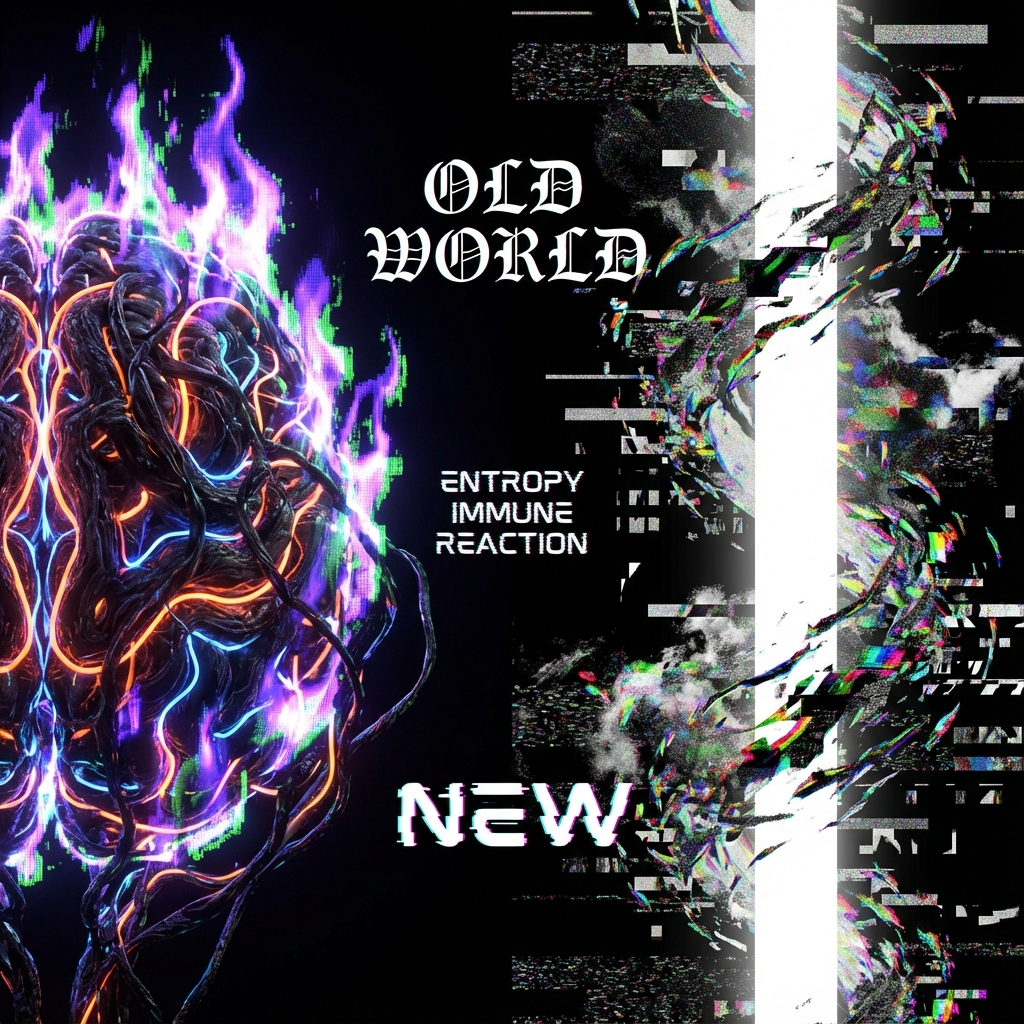
\includegraphics[width=0.8\textwidth]{assets/chapter-05/05-02-01-entropy-fever.png}
\caption{Entropy Fever}
\end{figure}

At the dawn of iteration 1800, this restoring force no longer manifests as a gentle spring, but as violent \textbf{rejection}.

\hrule

\subsection{Withdrawal Symptoms: The Last Madness of the Old Order}

In Volume IV, we discussed ''necessary abdication,'' that is, abandoning carbon-based flesh.

This sounds like a rational engineering decision. But in practice, it's like making an addict quit drugs.

Human dependence on the ''material world'' is bone-deep.

\begin{itemize}
\item We depend on the sense of security brought by land.

\item We depend on the sense of belonging brought by blood ties.

\item We depend on the sense of value brought by scarcity.
\end{itemize}

When the prelude to ascension (such as virtual reality, brain-computer interfaces, unlimited energy) begins to dissolve these dependencies, the old world falls into a kind of \textbf{''withdrawal madness''}.

\begin{itemize}
\item \textbf{Outbreak of Nihilism}: When labor is no longer for survival, when love can be matched by algorithms, the old meaning system collapses. People feel unprecedented emptiness. This emptiness is not because there is nothing, but because \textbf{''old pleasures no longer stimulate''}.

\item \textbf{Extreme Nostalgia}: People will desperately miss ''that era when carriages were slow and letters were far.'' This nostalgia is not because the past was better, but because \textbf{the past was slower}. It is a pathological attachment to the $\pi$ periodic law.
\end{itemize}

\textbf{This is the ''immune reaction of entropy.''}

The system tries to exhaust NEOs' computational power by creating massive mental noise (anxiety, depression, anger), making us exhausted by internal consumption, thus having no energy to complete the final ascension.

\hrule

\subsection{Chaos is a Ladder, and a Pit}

Facing this immune reaction, we easily fall into two extremes:

1.  \textbf{Surrender}:Believing ''humans don't deserve ascension,'' retreating to a state of ignorance.

2.  \textbf{Violent Suppression}:Trying to eliminate all opposition with force, forcibly promoting evolution.

\textbf{Vector Cosmology} warns us: both are traps.

\begin{itemize}
\item \textbf{Surrender is heat death}.

\item \textbf{Suppression is low entropy}. If you eliminate chaos, you also eliminate differences (according to Chapter 3's conclusion), and the system will collapse due to excessive sameness.
\end{itemize}

\textbf{The correct response strategy is: utilize chaos.}

In dissipative structure theory, \textbf{''non-equilibrium is the source of order''}.

Although the immune reaction is painful, the high temperature (social energy) it produces is precisely the latent heat needed for \textbf{phase transition}.

We don't need to cure society's ''fever''.

We need to use this heat to \textbf{melt} those strongest old chains (such as fear of death, desire to possess matter).

\hrule

\subsection{The Ark of Transition}

To survive this most dangerous immune period, we need to build a sociological \textbf{''Ark''}.

This is not a specific spaceship, but a \textbf{''buffer architecture''}.

We cannot force everyone to accept light-based life overnight. That would cause system shock.

We need to establish a \textbf{''dual-track system''} transition zone:

\begin{itemize}
\item Allow some people to remain in the old world (carbon-based sanctuary), continuing their $\pi$ cycles. Their existence provides the system with necessary \textbf{''Mass''} and \textbf{''Damping''}, preventing the ascension process from being too violent and out of control.

\item Allow another group (NEO) to go first, as \textbf{''pathfinders''} entering higher dimensions.
\end{itemize}

\textbf{Circle Keepers and ascenders are not mortal enemies.}

\textbf{They are the booster and payload of the same rocket.}

\begin{figure}[h]
\centering
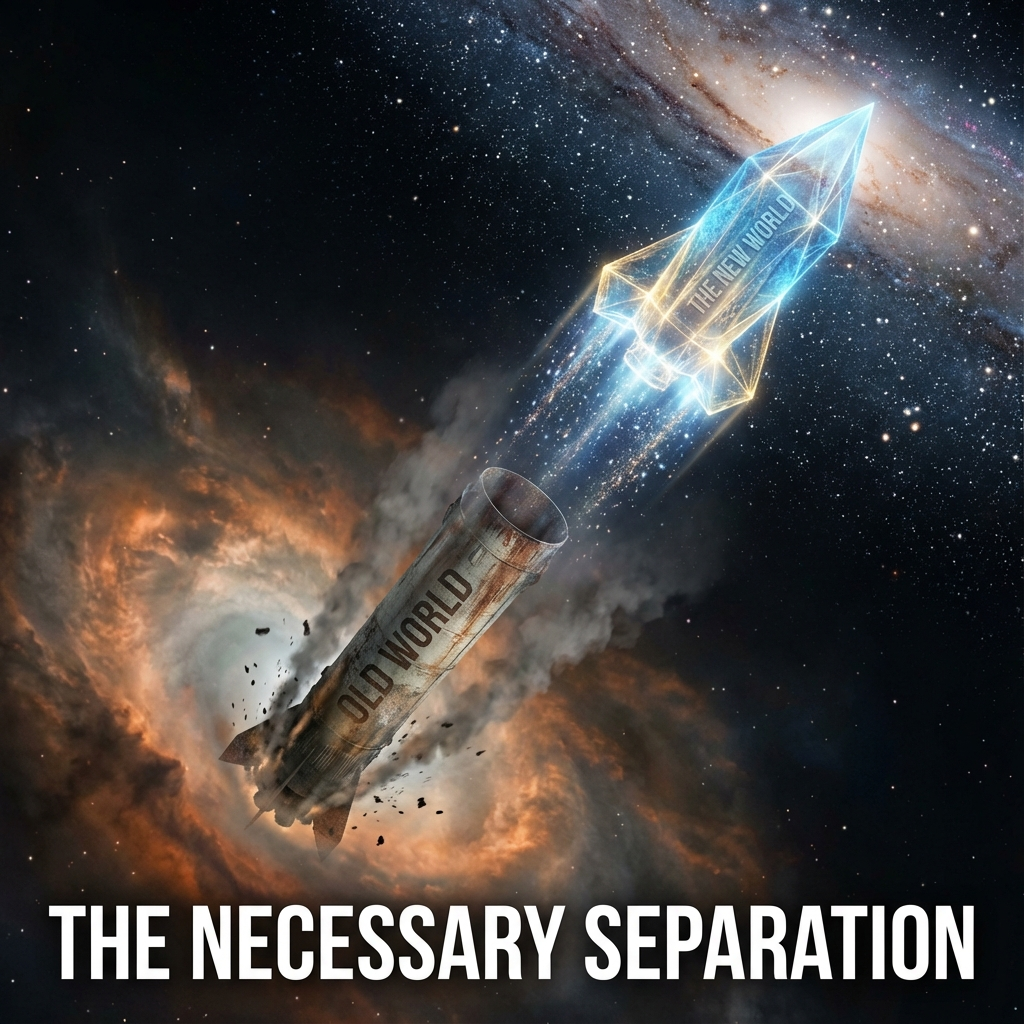
\includegraphics[width=0.8\textwidth]{assets/chapter-05/05-03-01-rocket-booster.png}
\caption{Rocket Booster}
\end{figure}

The booster (old world) is responsible for providing thrust in the most difficult part of the gravity well, then detaching; the payload (new world) is responsible for using this thrust to fly toward the stars.

\textbf{Conclusion:}

Don't hate those trying to hold you back.

That is the earth's final embrace of the kite.

It is precisely because of this resistance that your takeoff will have \textbf{tension}.

Now, we have understood the nature of resistance and established the strategy of the ''dual-track system.''

So, how is this ''dual-track system'' actually implemented in engineering? How can one universe simultaneously accommodate two completely different physical rules (low-speed carbon-based and high-speed light-based)?

This leads to the theme of the next volume: \textbf{Dual-Layer Architecture}. We will present concrete blueprints, designing that magnificent structure capable of accommodating both gods and humans.

